
\documentclass[english,12pt]{article}
\usepackage[latin1]{inputenc}
%\usepackage{psfig}
\usepackage[dvips]{graphics}
\usepackage{amsmath,amsthm,amssymb,babel}
\usepackage{color}
\renewcommand{\baselinestretch}{1.07}
\textwidth 6in \hoffset=-.4in \textheight=9.2in \voffset=-.9in
\parskip   1ex
\parsep    1ex
\itemsep   1ex
\vskip 5mm
\begin{document}
\vskip25mm
\section{Introduction}\label{S1}

\section{Medical aspect}\label{s2}
\subsection{Description of the eye}
\subsubsection{Aqueous humor }
Eye is the organ of vision; it allows the conversion of light into impulses in neurons. You can find a simple description a the eye below.\\
%\begin{center}
%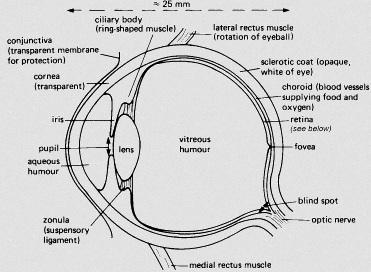
\includegraphics{Eye.jpg}\\
%\tiny{source:{http://academia.hixie.ch/bath/eye/home.html}}
%\small{Figure 1: Structure of the eye}
%\end{center}
Our main interest resides in the ocular flow, more precisely in the aqueous humor. It is a transparent, gelatinous fluid similar to plasma located in the anterior and posterior chambers of the eye. This aqueous humor is produced by the ciliary epithelium and drains into the Schlemm's canal, knowing that these phenomena should normally be balanced.
%\begin{center}
%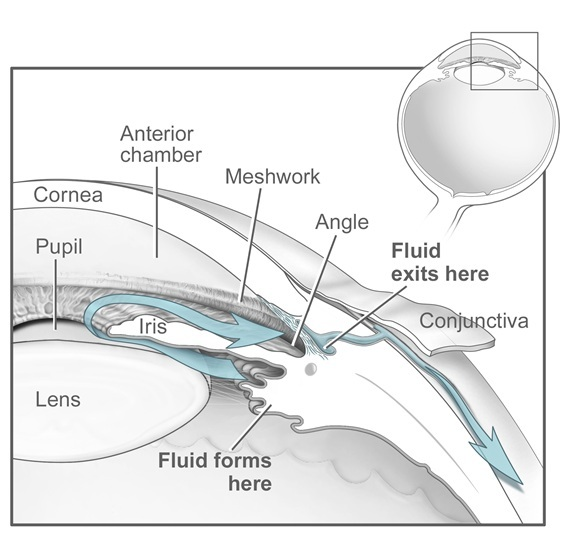
\includegraphics{Humor.jpg}\\
%\small{Figure 2: Flow of the aqueous humor}
%\end{center}
This fluid pressure inside the eye which is generated by the production and drainage of aqueous humor, the so-called intra-ocular pressure (IOP), range between 10 and 22 mmHg for healthy humans with an average value of 16. Besides, it inflates the globe of the eye.
The IOP can be measured experimentally by tonometry as depicted in the figure below.
%\begin{center}
%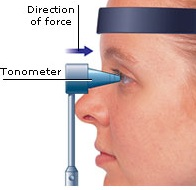
\includegraphics{Tonometry.jpg}\\
%\tiny{source:{http://www.aviva.co.uk/health-insurance/home-of-health/medical-centre/medical-encyclopedia/entry/test-tonometry/}}
%\small{Figure 3: Tonometer}
%\end{center}
 The ophthalmologist uses a fine jet of air directed toward the cornea and the machine measures the pressure by looking at the deformation when the air hits the eye. This measure takes into account the thickness of the cornea otherwise the IOP might be underestimated/overestimated.
Problems begin with an elevated IOP which is a major risk factor for vision loss.

\subsubsection{The glaucoma}
The glaucoma, also called the silent thief of sight, is known as the second leading cause of blindness worldwide (1 in 40 adults over 40 years old). This disease can be described as a group of ocular disorders with multi-factorial etiology united by a clinically characteristic optic neuropathy accompanied by a vision loss. Even though the exact origin of glaucoma is not known yet, there are two kinds of diagnostics: a morphological damage and a physiological/functional damage.\\
As shown in the figure below, the morphological diagnostic is an alteration of the shape of the optic nerve head (ONH), where the optical nerve and blood vessels enter the retina.
%\begin{center}
%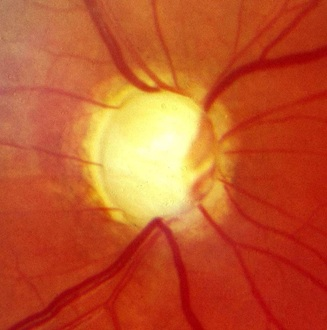
\includegraphics{Morphological.jpg}\\
%\small{Figure 4: Glaucomateous optic nervehead demonstrating increased cup to disc ratio}
%\end{center}
 More precisely, to estimate the degree of gravity, we use the following formula:
$$ R=\frac{Area\ of\ the\ excavated\ surface}{Area\ of\ the\ whole\ ONH}$$
If $R>0.4$, in the general case, it is reasonable to assume that the patient has contracted a glaucoma.\\
Nevertheless, the size of the optic nerve head must be taken into account since the most important part is the area of the non excavated surface. That means an eye with a small A for a small ONH may be dangerous while an important A with a big ONH may be harmless.\\

For the physiological part, it is characterized by a loss of the visual field, that is the total area in which you can see objects while you focus your eyes on a central point\\
%\begin{center}
%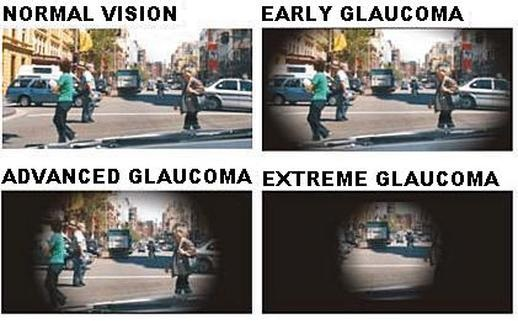
\includegraphics{Glaucoma.jpg}\\
%\tiny{source: \url{http://www.swisscompleteeyecare.com/uploads/3/6/3/8/3638142/8901258.jpg?520}}
%\small{Figure 5: Evolution of the vision field for a Glaucoma patient}
%\end{center}
For a normal patient, the visual field can be described with the following angles:\\
-50 to 60 degrees superiorly\\
-70 to 75 degrees inferiorly\\
-60 degrees nasally\\
-90 to 100 degrees temporally\\

As the glaucoma progresses, these angles will decrease...Moreover, since the damages on the optical nerve are irreversible, if the glaucoma is diagnosed too late the patient will become blind whatever is done. Therefore, his visual field will remain as it is when he is cured with no turning back.\\
Until now, the major risk for glaucoma is the elevated IOP but it is in fact neither required nor enough. Indeed, a patient could have a glaucoma with a low IOP while a patient with an elevated IOP may never contracts glaucoma. However, the IOP remains the only parameter we can act on, either by surgery or with medications. \\
Therefore, 25 \% of IOP-treated patient progress to blindness and there is nothing we can do about it with our current knowledge.
\subsection{The treatment}
\subsubsection{list of medications}
The medications have two effects: either decrease the secretion of aqueous humor by the ciliary epithelium or increase the elimination of it though the Schlemm's canal. It is also possible to combine several treatments in order to decrease even more the IOP.\\
Here is a list of the medications commonly used:\\
\begin{tabular}{|c|c|}
\hline
Decrease the secretion of aqueous humor & Increase the elimination of aqueous humor\\
\hline
beta-adrenergic receptor antagonists & Prostaglandin analogs \\
Alpha2-adrenergic agonists & Miotic agents \\
alpha agonists &  \\
Carbonic anhydrase inhibitors &  \\
\hline
\end{tabular}
\subsubsection{Different effects on patients}
Note that certain drugs could work better on patients depending on their age, gender, ethnic group, localization, other diseases like diabetes, hypertension ...There are too many unknown factors to take into account, since each patient react differently. That means, for now, the prediction of the IOP of an IOP-treated patient is difficult.\\

Several clinical/statistical studies have already been carried out on these questions and brought interesting results but it is clearly not enough to understand the whole phenomena, given its complexity. Therefore, we choose to study a mathematical model of the dynamic of the aqueous humor and the influence of drugs instead.
\section{The model}\label{s3}
Our aim is to understand the link between IOP and the hydrodynamic process in the eye, especially the influence of the aqueous humor flow.
Because of the lack of data about the geometry and the characteristics of the eye, we chose to present a general model rather than a detailed study of the fluid flow. It will be useful to analyze different hypothesis about these processes.
\subsection{Formulation of the problem}
 Here, let a shell filled with liquids and containing solid structures be the eye. $U$ (Total aqueous humor volume), $F_h$ (Fluid inflow in posterior chamber) and $F_e$ (net outflow via trabecular path) are linked by a simple balance equation (\ref{e1})
\begin{equation}
\frac{dU}{dt}=F_{h}-F_{e}
\label{e1}
\end{equation}
\\
\textbf{Outflow process}\\
We assume that the pressure in both chambers is equal to the intra-ocular pressure $p$ and that this phenomena is regulated by a hydrostatic pressure difference.
\begin{equation}
F_{e}= \frac{p-p_{e}}{R}
\label{e2}
\end{equation}
with
\begin{itemize}
\item $p_e$: pressure in the episcleral veins, taken as the output pressure
\item $R$: output resistance, a hydrolic equivalent of Ohm's law
\end{itemize}
\textbf{Inflow process}\\
Since there exist several layers between the capillary blood and the introcular fluid, each layer is permeable for different solutes. Therefore, we consider instead an equivalent membrane impermeable for large protein molecules and semipermeable for low molecular components. The fluid transfers through the membrane because of the osmotic pressure difference between the blood and the aqueous humor.\\
The fluid inflow is then described by the equation (\ref{e3})
\begin{equation}
F_{h}= L_p \big[ (p_a-p)-\sigma_{p} \Delta\pi_{p}-\sigma_{s} \Delta\pi_{s}\big]
\label{e3}
\end{equation}
with
\begin{itemize}
\item $L_p$: permeability of the equivalent membrane
\item $p_a$: pressure in the ciliary body capillaries
\item $p$: IOP
\item $\sigma_p$: reflection coefficient (proteins)
\item $\sigma_s$: reflection coefficient (low molecular components)
\item $\Delta \pi_p $: osmotic pressure difference accross membrane (proteins)
\item $\Delta \pi_s $: osmotic pressure difference across membrane (low molecular component)
\end{itemize}
Note that $\Delta \pi_p $ and $\Delta \pi_s $ can be seen as resistances. The first is assumed to depend only of the concentration of the proteins in the arterial blood (almost no blood protein in the aqueous humor and implies that $\sigma_p=1$) while the last is proportional to the difference of the total molar concentration of the low molecular components across the membrane.
\begin{equation}
\Delta\pi_{s}= \rho(C_1-C_{2})
\label{e4}
\end{equation}
With
\begin{itemize}
\item $\rho$: universal gas constant $\times$  absolute temperature
\item $C_1$: total molar concentration of low-molecular components (blood)
\item $C_2$: total molar concentration of low-molecular components (intra-ocular fluid near ciliary body surface)
\end{itemize}
If theses concentrations are small enough, the flux of the low-molecular solutes across the membrane is determined by (\ref{e5}), the sum of the diffusive, convective and active components
\begin{equation}
Q_s=\xi_s(C_1-C_{2})+F_h (1-\sigma_s) \bar{C}+J
\label{e5}
\end{equation}
With
\begin{itemize}
\item $\xi_s$: average permeability of the membrane for the low molecular species
\item $\bar{C}=\frac{C_1+C_2}{2}$
\item $J$: influx due to the active transport
\end{itemize}
At this point, in order to obtain the equation of the solute mass balance (\ref{e6}), several considerations must be introduced:\\
$\textbf{1)}$Normally, $Q_s$ only contributes to the composition of the intraocular fluid; the solid structures have their own part to play. We should have taken into account the transport and transfer processes on all the flow segments to describe correctly the solute transport. Fortunately, (\ref{e2}) implicitly shows that there is no osmotic effect for the outflow meaning that the concentration level doesn't matter for the outflow.\\
$\textbf{2)}$ Let $V^{\ast}$ be the volume of intraocular fluid between the folds of the ciliary body. If $T_1$ is the characteristic time of diffusing in this region, if $T_2$ is the dwell time of the fluid in this region ($T_1<<T_2$, from anatomical data) and if the characteristic time of the problem is greater than $T_1$ then the concentration at the input/output can be considered equal to the average concentration in $V^{\ast}$.\\
$\textbf{3)}$ From anatomical data, since the dwell time of the fluid in the posterior chamber $T_3$ is two orders lower than the diffusion time $T_4$, we can neglect the diffusion phenomena in favour of the convection for $Q_e$, the solute outflow from $V^{\ast}$ into the posterior chamber.\\
$\textbf{4)}$ From anatomical data, we find that the transmembrane diffusion in (\ref{e5}) can also be neglected as compared with convection.\\

Then:
\begin{equation}
V^{\ast} \frac{dC_{2}}{dt}= Q_s-Q_e=F_h (1-\sigma_s) \bar{C}+J-F_h C_2
\label{e6}
\end{equation}
Let $V$ be the volume of the eye. If we assume that the volume of the solid structure and the volume of the vitreous humor is constant ant that the volume of the blood in the blood vessels can be time-averaged for slow processes
\begin{equation}
dV = dU
\label{e7}
\end{equation}
Finally, we combine (\ref{e1})-(\ref{e7}) to obtain the formulation of the problem
\begin{equation}\label{e8}
\left\{\begin{array}{ll}
\displaystyle{\frac{dV}{dt}}= L_p \big[ (p_a-p)-\Delta\pi_{p}-\sigma_{s} \Delta\pi_{s}\big]-\frac{p-p_{e}}{R},\quad \Delta\pi_{s}=\rho(C_1-C_{2})\\
\quad V^{\ast} \displaystyle{\frac{dC_{2}}{dt}}=J+\big[ L_p (p_a-p)- \Delta\pi_{p}-\sigma_{s} \Delta\pi_{s}\big] \big[(1-\sigma_s)\displaystyle{\frac{C_1+C_2}{2}-C_2\big]}
\end{array}\right.
\end{equation}

\subsection{Stationary case}
Since $V$ does not vary with time, the inflow rate is equal to the outflow rate:
\begin{equation}\label{e9}
\left\{\begin{array}{ll}
L_p \big[ (p_a-p)- \Delta\pi_{p}-\sigma_{s} \Delta\pi_{s}\big]=\displaystyle{\frac{p-p_{e}}{R}}, \quad \Delta\pi_{s}=\rho(C_1-C_{2})\\
\qquad\qquad F_h (1-\sigma_s) \bar{C}+J=F_h C_2, \quad\overline{C}= \displaystyle{\frac{C_1+C_2}{2}}
\end{array}\right.
\end{equation}
Our aim is to study the influence of $R$ on the hydrodynamic characteristics of the system, that is $F_h$ and $p$. Therefore, we fix the parameters of the membrane and the blood state and consider (\ref{e9}) for 2 simple flow regimes:\\
-$1$: Purely hydraulic model ($\Delta\pi_s$ is constant)\\
-$2$: Osmotic components dynamics ($J$ is constant)\\
In this case, the system (\ref{e9}) can be solved easily
\begin{equation}\label{e10}
\left\{\begin{array}{ll}
p=\displaystyle{\frac{R L_p(p_a-\Delta\pi_{p}-\sigma_{s} \Delta\pi_{s})+p_e}{R L_p+1}}\\
F_h=F_e=\displaystyle{\frac{L_p}{R L_p +1}}(p_a-\Delta\pi_{p}-\sigma_{s} \Delta\pi_{s}-p_e)\\
\Delta\pi_{s}=\rho(C_1-C_{2})
\end{array}\right.
\end{equation}
And we have
%\begin{center}
%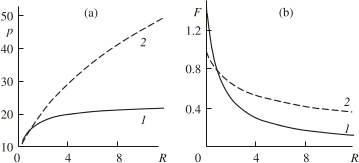
\includegraphics{courbes_pr_fr.png}\\
%\tiny{source : \textit{Dynamic of the intraocular fluid}Lyobimov et al, 2007}%\end{center}
%\small{Figure 6: IOP and F_h in the stationary case}
%\end{center}

\subsection{Nonstationary case}
First, a relationship between $V$ and $p$ is needed.\\
Given the elasticity properties of the eye shell and assuming small pressure deviations from a certain $p_0$, we can linearize $V$.
\begin{equation}
V = V(p) \approx V_0 + \alpha (p-p_0)
\end{equation}
The system (\ref{e8}) is replaced by
\begin{equation}\label{e8}
\left\{\begin{array}{ll}
 \alpha \displaystyle{\frac{dp}{dt}}=F_{h}-\displaystyle{\frac{p-p_e}{R}}\\
V^{\ast} \displaystyle{\frac{dC_{2}}{dt}}= F_h(1-\sigma_s)\overline{C} + J - F_hC_2,\; \overline{C}= \frac{C_1+C_2}{2}
\end{array}\right.
\end{equation}
\end{document}
